\documentclass{article} % For LaTeX2e
\usepackage{iclr2016_conference,times}
\usepackage{hyperref}
\usepackage{url}
\usepackage{graphicx}


\title{Paper Reading Report}


\author{Hu Jiyuan \thanks{ Student ID: 18215258, Class ID: 11} \\
School of Electronics and Information Technology\\
Sun Yat-sen University\\
Guangzhou, China \\
\texttt{hujy23@mail2.sysu.edu.cn} \\
}

\newcommand{\fix}{\marginpar{FIX}}
\newcommand{\new}{\marginpar{NEW}}

%\iclrfinalcopy % Uncomment for camera-ready version

\begin{document}


\maketitle

\begin{abstract} 
\footnote{I originally want to use ``\textsc{Requirements}'' here 
but this report is organized by the same \LaTeX{} template with the 
paper I read, I can't change the ``\textsc{Abstract}'' and the header.
``Under review as a conference paper at ICLR 2016''} 
Draw an outline for the paper and summarize the main idea of each part.
Quote sentences typical of a part that you can use in your own paper.
Quote sentences you find difficult to understand.
Record the bibliographic information of the paper 
(1) by following its documentation style and 
(2) in the Chicago style.
\end{abstract}

\section{Outline \& main idea}
\begin{figure}[h]
\begin{center}
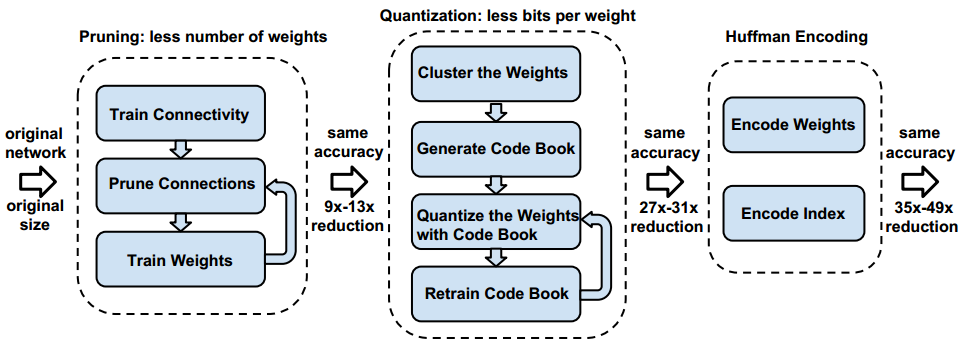
\includegraphics[width=\textwidth]{graphics/part1-overview.png} 
\end{center}
\caption{Main content of the paper I read}
\end{figure}

\subsection{Abstract} 

\textsc{Abstract} answers the following four questions: 
    \par What problems have people met?
    \par What's your solution?
    \par How does the solution work?
    \par How well does the solution work in comparison of existing solutions?

\subsection{Introduction}

\label{introduction}
\textsc{Introduction} first introduces the background and need of the 
neural networks compression solutions: reduce the storage and energy required 
to run inference on large networks. Then briefly describes their solutions in three
parts: pruning, trained quantization and Huffman coding.

\subsection{Network Pruning} 

\textsc{Network Pruning} shows how to prune the network. Neural networks 
have many connections, they prune the small-weight connections.

\subsection{Trained Quantization and Weight Sharing} 

\textsc{Trained Quantization and Weight Sharing} continues to compress 
the network by reducing the number of bits required to represent each weight, which 
is what called quantization. They use k-means clustering to find the weight that 
can be shared. 

\subsection{Huffman Coding} 

\textsc{Huffman Coding} is used in the purpose of encoding (or compression) 
the quantized weights and sparse matrix index generated by the former step.

\subsection{Experiments} 

\textsc{Experiments} are taken to show the performance of their solutions by 
comparing the network parameters and accuracy of several networks before and after 
their solutions are taken.

\subsection{Discussions} 

\textsc{Discussions} discuss the relationship between performance and 
configuration.

\subsection{Related Word} 

\textsc{Related Word} is the extension of the background description in 
section \ref{introduction}. It mainly tells us the neural networks are over-parametrized 
and introduce the typical methods taken to solve the problem by other people. 

\subsection{Feture Work} 

\textsc{Feture Work} denotes what they are going to do next: build software 
to complete the benchmarked test they does not finish because of the existing software 
does not support their solution. What's more, to build hardware (ASIC chip) to achieve 
their solutions.

\subsection{Conclusion} 

\textsc{Conclusion} concludes their steps, key performance and application 
scene of their solutions.

\subsection{References} 

\textsc{References} are in alphabetical order.

\section{Typical Sentences}

\subsection{To Address}

To address this limitation, we introduce “something”, some introduction.

Examples: To
address this limitation, we introduce “deep compression”, a three stage pipeline:
pruning, trained quantization and Huffman coding, that work together to reduce
the storage requirement of neural networks by 35× to 49× without affecting their
accuracy.

To achieve this goal, we present “deep compression”: a three stage pipeline (Figure 1) 
to reduce the storage required by neural network in a manner that preserves the 
original accuracy.

\subsection{Figure}

xxx is illustrated in Figure x.

Examples: Weight sharing is illustrated in Figure 3.

\section{Difficult Sentences}

While the \emph{pruned} network has been benchmarked on various hardware, 
the \emph{quantized} network with weight sharing has not, because off-the-shelf 
cuSPARSE or MKL SPBLAS library does not support indirect matrix entry lookup, nor is 
the relative index in CSC or CSR format supported. So the full
advantage of Deep Compression that fit the model in cache is not fully unveiled. 

\section{Bibliographic Information}

\subsection{Written by Myself}

\subsubsection{Style Used by the Author}
Han, Song, Mao, Huizi and Dally, William J. Deep compression: compressing 
deep neural networks with pruning, trained quantization and huffman coding. 
In \emph{International Conference on Learning Representations}, 2016

\subsubsection{Chicago Style}
Han, Song, Mao, Huizi and Dally, William J. ``Deep compression: compressing 
deep neural networks with pruning, trained quantization and huffman coding.'' 
\emph{International Conference on Learning Representations} (2016). https://arxiv.org/abs/1510.00149

\subsection{Standard Answer}

\subsubsection{Style Used by the Author}

This is in-text citation, see \citet{han2015deep}.

And the following is bibliography:

\bibliography{iclr2016_conference}
\bibliographystyle{iclr2016_conference}

Generated by the ICLR \LaTeX{} template itself.

\subsubsection{Chicago Style}

Han, Song, Huizi Mao, and William J. Dally. ``Deep compression: Compressing deep 
neural networks with pruning, trained quantization and huffman coding.'' \emph{arXiv 
preprint arXiv:1510.00149} (2015).

Generated by Google Scholar.

\end{document}
